\section{Rethinking Speculate--Verify for Deep Research Agents}
\label{sec:motivation}
% Existing speculate--verify frameworks for agents typically apply a \emph{uniform} speculation strategy across all actions, either by (i) reducing reasoning depth (e.g., skipping explicit reasoning) or (ii) reducing model capacity (e.g., using a smaller speculator). While effective in some settings, this approach ignores a key property of deep research agents: \emph{actions are heterogeneous in their reasoning demands}. In this section, we present empirical evidence showing that Search and Visit actions exhibit fundamentally different sensitivities to reasoning depth and model capacity. These findings motivate an \emph{action-aware speculation} design. We also analyze the trade-offs in verification strategies, highlighting the need for approaches that go beyond action matching.

Existing speculate--verify frameworks typically apply a \emph{uniform} speculation strategy across all actions, either by (i) reducing reasoning depth (e.g., skipping explicit reasoning) or (ii) reducing model capacity (e.g., using a smaller speculator). While effective in some settings, this overlooks a key property of deep research agents: \emph{actions exhibit heterogeneous reasoning demands}. In this section, we provide empirical evidence that Search and Visit actions differ fundamentally in their sensitivity to reasoning depth and model capacity, motivating an action-aware speculation design. We further analyze verification trade-offs, highlighting the need to move beyond action matching.

\subsection{Speculation Under Action Heterogeneity}
We first examine the reasoning demands of different actions and then study how various speculation strategies affect the accuracy of drafting Search and Visit actions.

\begin{figure}
    \centering
    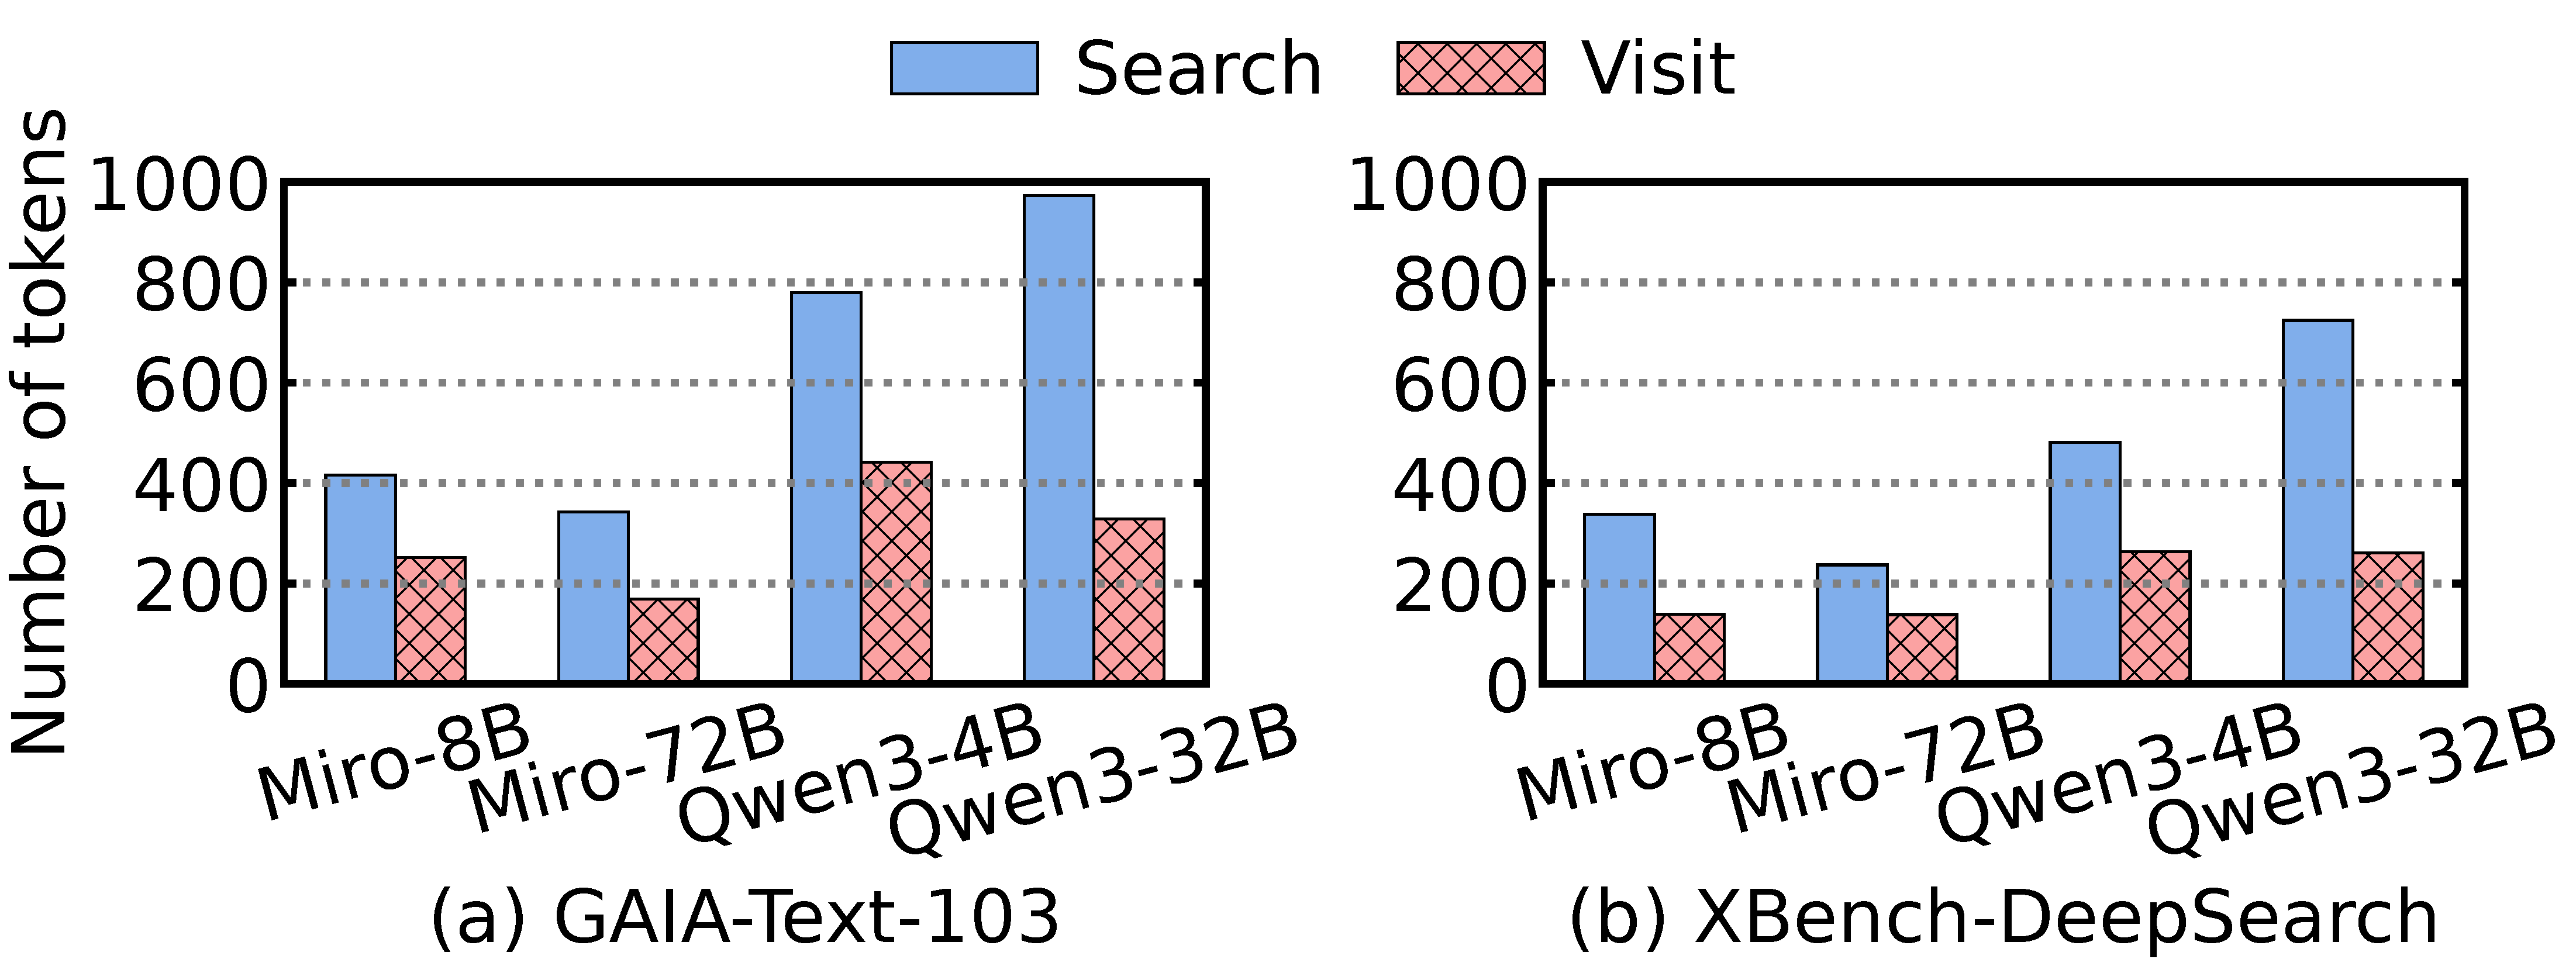
\includegraphics[width=\linewidth]{figs/token_count.pdf}
    \caption{Average reasoning length for generating Search and Visit actions across models and benchmarks. Search requires significantly longer reasoning than Visit.}
    \label{fig:motivation_tokens}
\end{figure}

\paragraph{Observation 1: Search actions involve longer reasoning traces than Visit.} 
Figure~\ref{fig:motivation_tokens} shows the average reasoning length before emitting an action. Across all models, Search consistently requires $1.65$--$2.95$$\times$ more tokens than Visit, indicating that query formulation inherently demands more deliberation than webpage selection. Therefore, Search actions carry stronger reasoning requirements.


% \paragraph{Observation 2: Effective speculation requires different strategies for Search and Visit.} 
% We measure alignment of the generated action using lightweight speculative methods with an Oracle agent (large model with full reasoning). Two representative strategies are compared: a small language model (SLM) with explicit reasoning, and a large language model (LLM) that skips reasoning 

% As shown in Figure~\ref{fig:motivation_alignment}(a),
% for Search actions, the small reasoning model consistently produces queries more aligned with the Oracle than the large model without reasoning, quantified via embedding-based cosine similarity~\cite{reimers-2019-sentence-bert}. Therefore, explicit reasoning is critical for query quality, even with reduced model capacity.
% In contrast, Figure~\ref{fig:motivation_alignment}(b--c) demonstrates that, to generate Visit actions, the large model skipping reasoning aligns more closely with the Oracle in both URL selection and extraction instruction. This indicates that deliberative reasoning is less crucial for Visit, where fast, pattern-based selection with large model capacities suffices.

\paragraph{Observation 2: Effective speculation strategies differ across actions.}
We measure the alignment of speculative actions with an Oracle agent (large model with full reasoning) using two representative strategies: a small language model (SLM) with explicit reasoning and a large language model (LLM) that skips reasoning.
As shown in Figure~\ref{fig:motivation_alignment}(a), for Search actions, the SLM with reasoning consistently produces queries more aligned with the Oracle than the LLM without reasoning, measured via embedding-based cosine similarity~\cite{reimers-2019-sentence-bert}. This indicates that explicit reasoning is critical for query quality even under reduced model capacity. In contrast, Figure~\ref{fig:motivation_alignment}(b--c) shows that for Visit actions, the LLM without reasoning aligns more closely with the Oracle in both URL selection and extraction instruction, suggesting that deliberative reasoning is less essential for Visit, where pattern-based selection benefits more from model capacity.
\begin{figure}
    \centering
    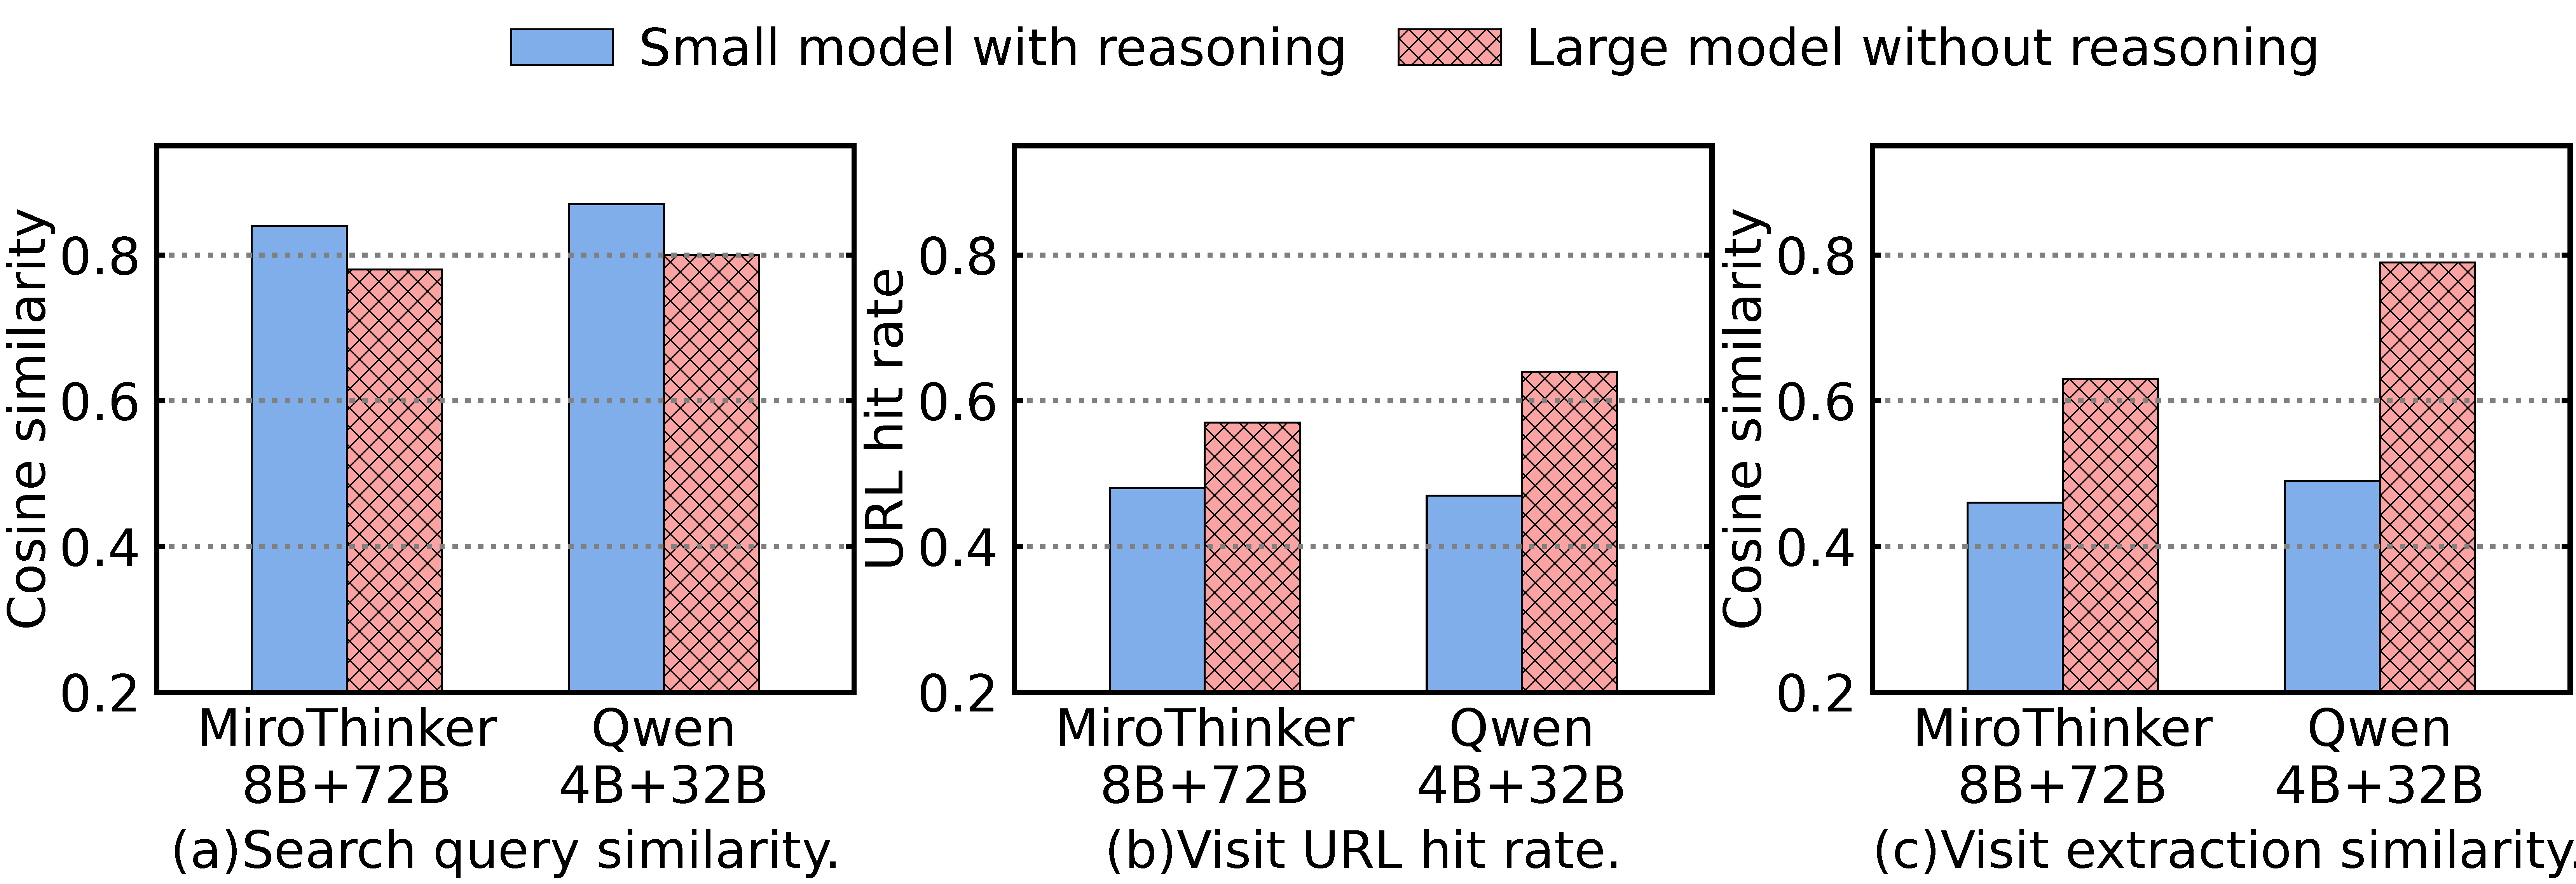
\includegraphics[width=\linewidth]{figs/motivation_similarity.pdf}
    \caption{Action alignment comparison of two speculative methods relative to the Oracle (large model with reasoning) when drafting Search and Visit. (a) The small reasoning model produces  queries more aligned with the Oracle than the large model without reasoning. (b--c) For Visit, the large model skipping reasoning achieves higher accuracy in both URL selection and extraction instruction.}
    \label{fig:motivation_alignment}
\end{figure}

\begin{table}[t]
    \centering
    \caption{End-to-end agent performance (pass@1 accuracy) on GAIA under action-level replacements.
We selectively replace the generation strategy for Search or Visit using lightweight methods.}
    \label{tab:action}
    {\small
    \begin{tabularx}{\columnwidth}{Xcc}
        \toprule
        Configuration & MiroThinker & Qwen3 \\
        \midrule
        LLM with Reasoning        & \textbf{63.11} & \textbf{29.13} \\
        \hdashline
        SLM with Reasoning for Search     & \textbf{63.11} & \textbf{29.13} \\
        LLM without Reasoning for Search  & 57.28 & 23.30 \\
        SLM without Reasoning for Search  & 55.34 &  22.33 \\
        \hdashline
        SLM with Reasoning for Visit      & 56.31 & 22.33 \\
        LLM without Reasoning for Visit   & \textbf{64.08} & \textbf{28.16} \\
        SLM without Reasoning for Visit  & 54.37 & 24.27 \\
        \bottomrule
    \end{tabularx}
    }
\end{table}


% To assess how different lightweight draft methods impact the end-to-end agent performance, we perform action-level interventions that selectively replace the generated action using a lightweight method, while keeping the remainder of the agent pipeline unchanged. We also consider a third option that combines both reduced model capacity and reasoning depth (SLM without reasoning).

% Table~\ref{tab:action} shows the results.
% Assigning small reasoning model to \textit{Search} preserves end-to-end accuracy, whereas 
% using a large model without reasoning degrades performance.
% Conversely, generating \textit{Visit} with a large model skipping reasoning achieves the best results, while another option leads to significant accuracy drops.
% Interestingly, although Figure~\ref{fig:motivation_alignment} demonstrates that the speculation cannot perfectly align with the Oracle at the action level, the end-to-end 
% accuracy can still be well maintained when right inference pathways are chosen for different actions.

To assess end-to-end effects, we perform action-level interventions that selectively replace Search or Visit generation with lightweight methods while keeping the rest of the pipeline unchanged. We also include another variant of speculation combining reduced capacity and reduced reasoning (SLM without reasoning).
Table~\ref{tab:action} shows that assigning an SLM with reasoning to \textit{Search} preserves overall accuracy, whereas using an LLM without reasoning degrades performance. Conversely, generating \textit{Visit} with an LLM without reasoning yields the best results, while alternative choices lead to significant accuracy drops. Although speculative actions do not perfectly align with the Oracle (Figure~\ref{fig:motivation_alignment}), 
end-to-end accuracy remains high because of the tolerance of approximation in reasoning models, as long as appropriate inference pathways are chosen per action.


% end-to-end accuracy remains high when appropriate inference pathways are chosen per action.



% \paragraph{Key insight: Search as System~2, Visit as System~1.}
% Taken together, these observations reveal a clear dichotomy between action types.
% We interpret this through the lens of dual-process theory.
% Search aligns with System~2 behavior: it requires deliberative reasoning to bridge the gap between an underspecified research objective and an effective query.
% In contrast, Visit aligns with System~1 behavior: given a set of candidates, selection and extraction rely primarily on fast, intuitive pattern recognition encoded in the model's parametric knowledge.
% This distinction provides a principled foundation for action-aware speculation.

\paragraph{Key insight: Search as System~2, Visit as System~1.}
These results reveal a clear action-level dichotomy. Viewed through dual-process theory, Search exhibits System~2 behavior, requiring deliberative reasoning to translate underspecified research goals into effective queries. Visit aligns with System~1 behavior, where selection and extraction primarily rely on fast, pattern-based recognition encoded in model parameters. This distinction provides a principled foundation for action-aware speculation.


% \subsection{Verification Beyond Action Matching}
% Speculation alone is insufficient for reliable speedups; verification is critical to prevent error propagation. Existing approaches typically verify speculative actions via exact or approximate action matching against the base model output. However, this strategy has two limitations.

% First, defining action equivalence is non-trivial. Exact matching is overly restrictive: 
% semantically equivalent Search queries may differ at the token level, leading to unnecessary rejection. 
% Approximate matching often requires additional modules (e.g., embedding models) and threshold tuning, complicating systems design.

% Second, verification usually requires the base model to complete its reasoning trace, placing it on the critical path and limiting latency reduction. More aggressive speculate-verify designs~\cite{guan2025dynamic} allow speculation to continue multiple steps for parallel verification, but failure in the middle requires rolling back all speculative steps, wasting computation.
% Therefore, achieving better accuracy-efficiency trade-offs demands verification strategies that go beyond simple action matching.

\subsection{Verification Beyond Action Matching}
Speculation alone is insufficient for reliable speedups; verification is essential to prevent error propagation. Most existing methods verify speculative actions via exact or approximate matching with the base model output, but this has two limitations.
First, action equivalence is hard to define. Exact matching is overly restrictive, as semantically equivalent Search queries may differ token-wise, causing unnecessary rejection, while approximate matching often requires additional modules (e.g., embedding models) and threshold tuning.
Second, verification typically places the base model's full reasoning trace on the critical path, limiting latency gains. More aggressive designs~\cite{guan2025dynamic} allow multi-step speculation with parallel verification, but failures in the middle require rolling back all following speculative steps, wasting computation. Achieving better accuracy-efficiency trade-offs therefore requires verification strategies beyond simple action matching.
 





\iffalse

\subsection{Speculation Under Action Heterogeneity}

To reduce the cost of agents, existing systems typically adopt two forms of speculation: reducing reasoning or reducing model capacity by using smaller models.
These strategies are commonly applied uniformly across all actions.
In this section, we examine how they affect different action types, and show that their effectiveness is highly action-dependent.
We present a set of empirical observations that motivate our key hypothesis that different actions exhibit different sensitivities to reasoning and model capacity.

\begin{figure}
    \centering
    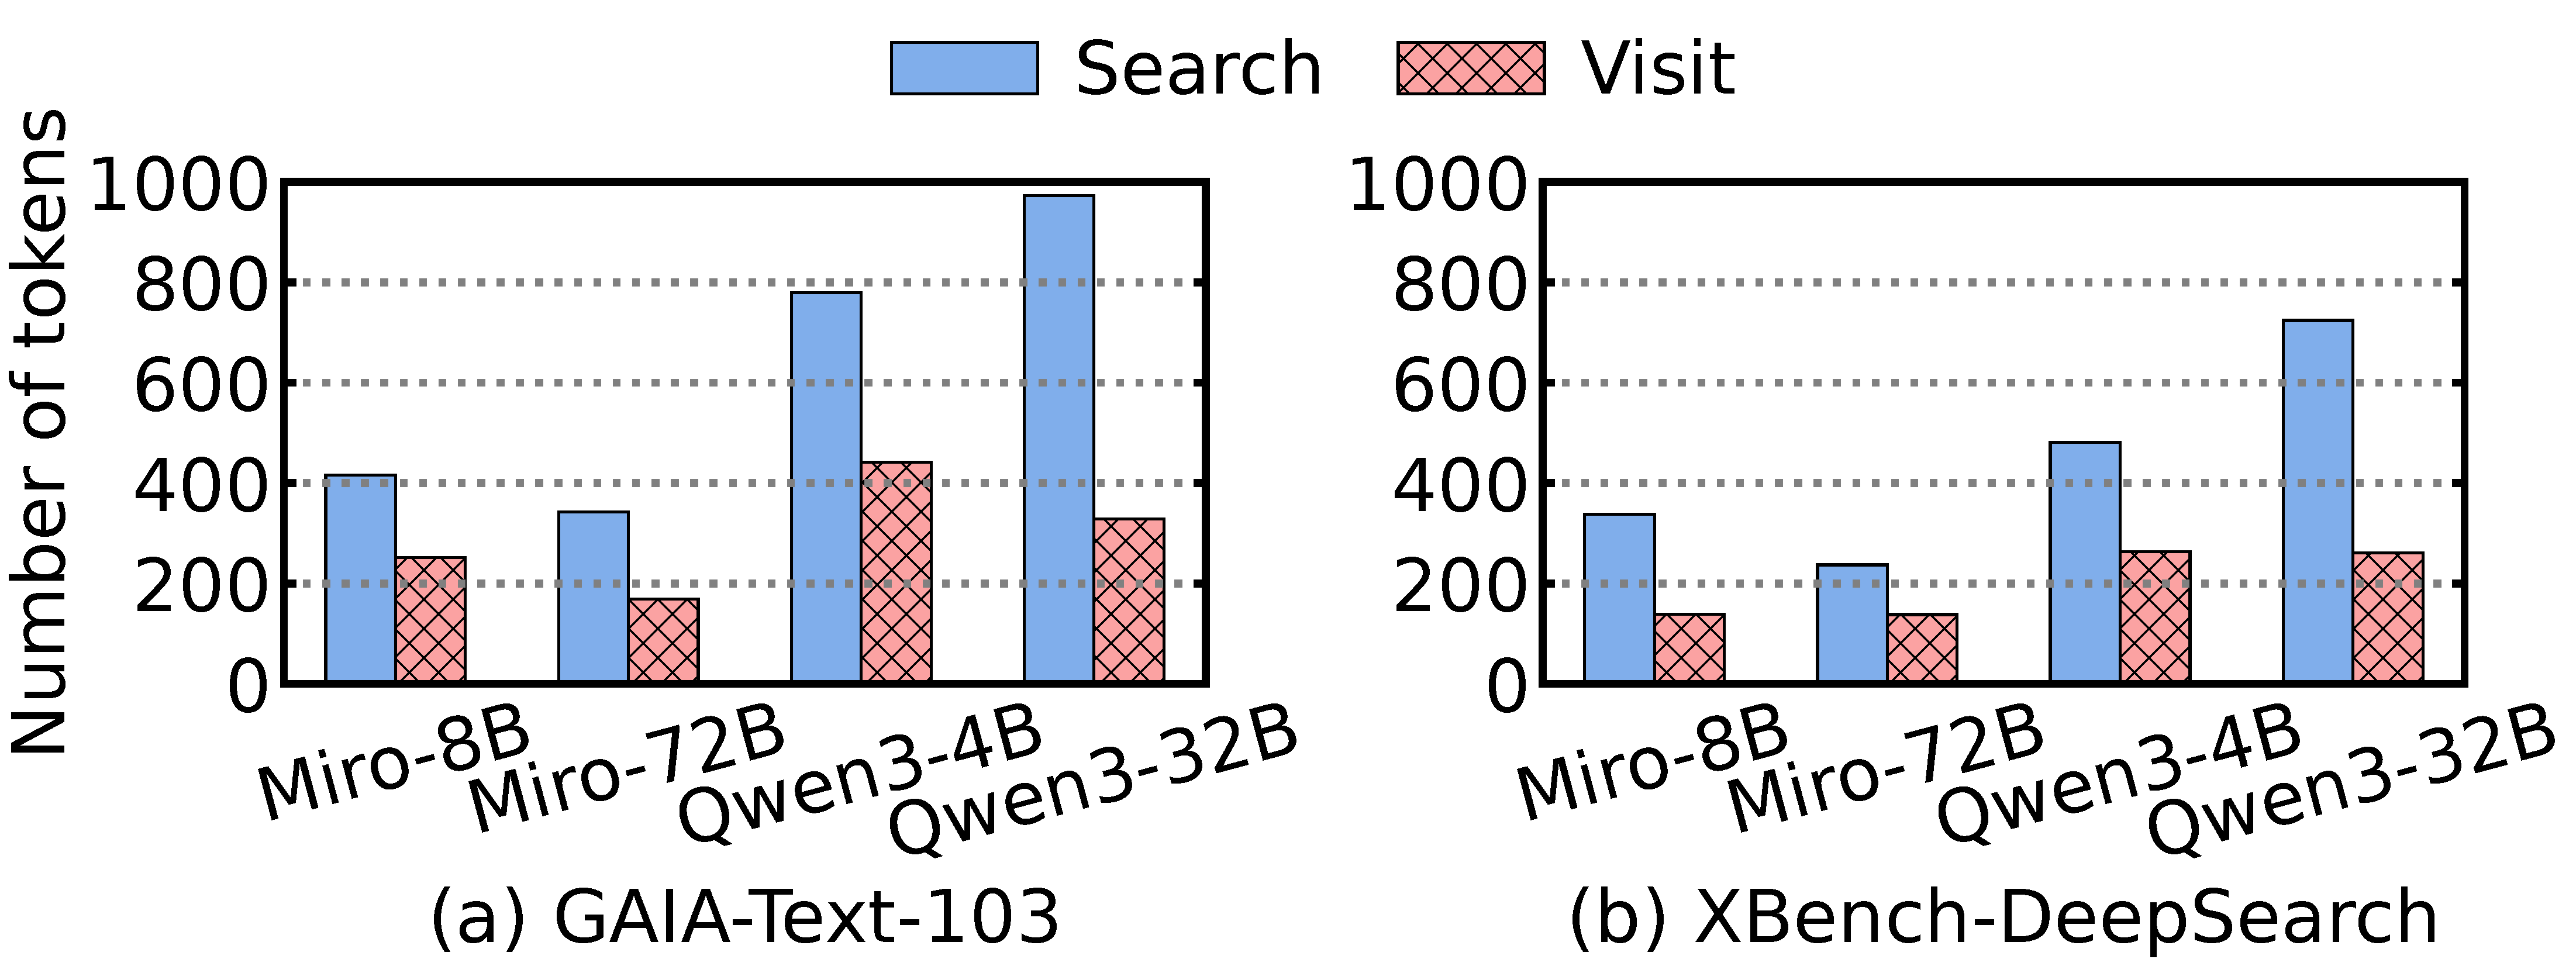
\includegraphics[width=\linewidth]{figs/token_count.pdf}
    \caption{Comparison of reasoning length for generating \textit{Search} and 
    \textit{Visit} actions on different benchmarks. \textit{Search} requires longer reasoning length than \textit{Visit}.}
    \label{fig:motivation_tokens}
\end{figure}

\paragraph{Observation 1: Search is preceded by longer reasoning traces than Visit.}
We observe a consistent gap in the amount of pre-action generation across action types.
As illustrated in Figure~\ref{fig:motivation_tokens}, the number of tokens produced before emitting a \textit{Search} action is consistently larger than that before a \textit{Visit} action across models and benchmarks.
This result indicates that models tend to spend more tokens before committing to Search than Visit within the same deep research workflow.

% \bt{Search naturally needs more reasoning tokens than visit.}

\begin{figure}
    \centering
    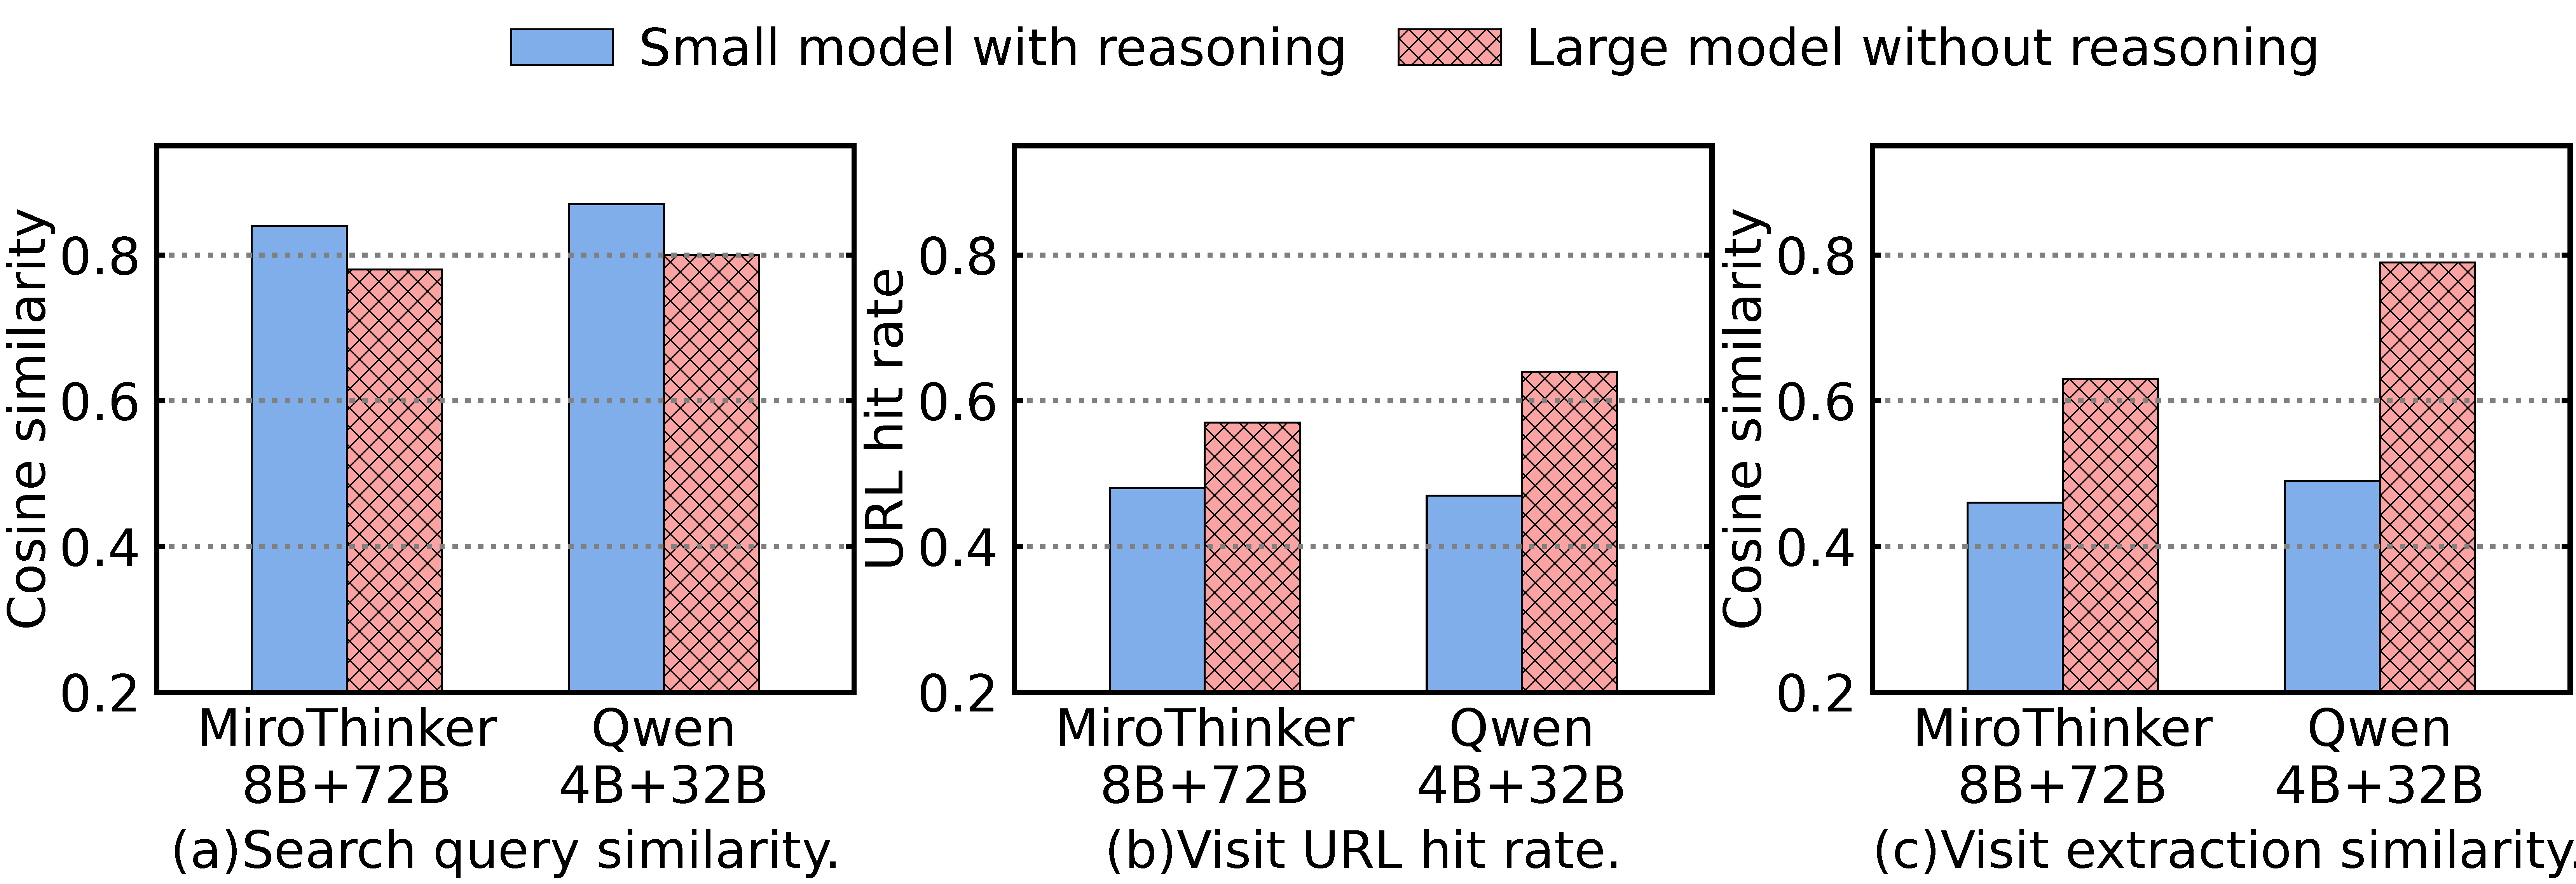
\includegraphics[width=\linewidth]{figs/motivation_similarity.pdf}
    \caption{Action alignment comparison of two lightweight methods relative to the Oracle (large model with reasoning). (a)(c) For Search queries and Visit extraction infos, we use the embedding-based cosine similarity between the generated query and the Oracle’s query. (b) For Visit URLs, alignment is evaluated using the direct hit rate against the Oracle’s selection.}
    \label{fig:motivation_alignment}
\end{figure}

\paragraph{Observation 2: Asymmetric Alignment Requirements for Search and Visit.}
We find that the requirements for maintaining behavioral alignment with the Oracle (Large Model with full reasoning) are fundamentally different for Search and Visit actions.

Specifically, for Search actions, a small model with reasoning aligns more closely with the Oracle than a Large Model without reasoning. We measure alignment by calculating the cosine similarity of the embeddings of the generated search queries with a a pre-trained embedding model. As shown in Figure~\ref{fig:motivation_alignment}(a), across the two model series, small model with reasoning can generate quereis that are more consistent with the reference compared with large model without reasoning.

In contrast, for Visit actions, a Large Model skipping reasoning aligns more closely with the Oracle than small model with reasoning. We evaluate alignment through two specialized metrics for the the target URL selection and the information extraction instruction in the visit arguments. For URL selection, we measure the direct hit rate against the Oracle’s chosen link. For extraction instructions, we compute the cosine similarity between the embeddings of the generated text and the Oracle’s reference, mirroring our evaluation of Search queries. As illustrated in Figure~\ref{fig:motivation_alignment}(b)(c), the alignment peaks when the large model is used.

\begin{table}[h]
    \centering
    \caption{End-to-end accuracy on gaia-text-103 under action-level replacements.
We selectively modify the generation strategy for \textsc{Search} or \textsc{Visit} while keeping the rest unchanged.}
    \label{tab:placeholder_label}
    \begin{tabular}{ccc}
        \toprule
        Configuration & MiroThinker& Qwen3 \\
        \midrule
        Large Model                 & \textbf{63.11} & \textbf{29.13} \\
        Small Model For Search      & \textbf{63.11} & \textbf{29.13} \\
        Small Model For Visit       & 56.31 & 22.33 \\
        Skip Reasoning For Search   & 57.28 & 22.33 \\
        Skip Reasoning For VISIT    & \textbf{64.08} & \textbf{28.16} \\
        Small + Skip  For Search    &  &  \\
        Small + Skip  For VISIT    & 54.37 &  \\
        \bottomrule
    \end{tabular}
\end{table}

\paragraph{Observation 3:}
We take action-level interventions that replace only the action generation module while keeping the rest of the agent pipeline unchanged.
As shown in Table~\ref{tab:placeholder_label}, assigning reasoning to \textsc{Search} preserves end-to-end accuracy, while skipping reasoning for \textsc{Visit} does not hurt the performance. These results indicate that once actions are generated under appropriate inference pathways, maintaining accuracy does not hinge on enforcing strict per-step alignment.

\paragraph{Key Insight: Search as System~2, Visit as System~1.}
Building upon these observations, we hypothesize that Search and Visit place fundamentally different demands on a model's inference process. We frame this distinction through the lens of dual-process theory: Search aligns with System 2 behavior, where deliberative reasoning is essential to bridge the "reasoning gap" between an underspecified research goal and an effective query. Conversely, Visit corresponds to System 1 behavior; once candidate results are presented, the selection and extraction process is more direct, relying on the model’s internal parametric knowledge rather than explicit logical deduction.

\subsection{Verification Beyond Exact Action Matching}

\noindent \textbf{Principle~2: Lightweight semantic verification.}
Rather than enforcing strict action-level equivalence at every step, high end-to-end accuracy can be achieved through lightweight semantic verification.
Specifically, each generated action can be evaluated by a full-capacity model using a coarse-grained consistency check with respect to the overall reasoning trajectory, without requiring exact matching to a reference output.
As long as the action is deemed semantically consistent, it can be accepted, reserving full regeneration for cases where substantial deviation is detected.

\fi


% \noindent \textbf{Principle~1: Heterogeneous Action Generation.}
% This System~1/System~2 distinction suggests a simple design principle: inference should be heterogeneous across actions.
% Actions that align with System~2 behavior should be generated with explicit reasoning to support deliberative decision making, while System~1 actions can be generated directly by a strong model without additional reasoning.
% Concretely, this motivates assigning reasoning, even with a smaller model, to \textsc{Search}, and executing \textsc{Visit} with a full-size model while skipping explicit reasoning.